\chapter{Introduction}
\label{sec:introduction}

\section{Motivation}
\gls{IR} systems become more important not only due to their use in Internet and digital libraries, but also because the majority of companies organize their activities around information and depend on digital documents. Finding the right information brings value to the business, and failing to do so usually leads to losses.\\

Certain factors influence  the performance of search applications. On one hand, it is the constantly growing problem of information overload. On the other, it is the peculiarities of humans users which have to be taken into consideration. \gls{IR} systems need to adapt to their users, and to their information need. \\

\begin{itemize}
\item \textbf{Human behavior}. Users searching for information usually submit queries composed of a few keywords only, as shown in studies~\cite{98usersSearchBehavior}.  For example, the average web users enter around 3 words per query\footnote{\url{http://www.hitwise.com/us/press-center/
press-releases/google-searches-apr-09}, accessed December, 2010}. The search application performs exact matching between the submitted keywords, and the document set it searches through, and often returns a long list of results. When searching with short queries, the focus of users is unclear, and the missing information contributes to long result lists containing many irrelevant hits. Users without domain expertise are not familiar with the appropriate terminology, and therefore they don't submit the right query terms with respect to relevance or specialization. Another issue is the ambiguity of words, in the cases when words have more than one meaning. When relevant documents contain words that are semantically relevant to the queries but not the same (synonyms), they will not be judged relevant. As a consequence, search results will not fit the information needs of users.  
\item \textbf{Manual processing of results}. When a large number of matching documents is returned as a search result, only some of the documents can be read, due to human limitations in information processing, and time constraints (users want to find information quickly). Human users need to narrow down the search iteratively by reformulating the query, since it is unclear in which context their queried words are used, and which words could be useful to focus the search. This reformulation can be a frustrating and time consuming process.
\item \textbf{Information need}. Search applications that implement the keyword search paradigm (or full-text search) are broadly accepted by users; however, the challenge for the next years is the development of search solutions that reflect users' context ("what the user meant" versus "what the user entered as a query"). In other words, solutions that are able to:   
\begin{inparaenum}[\itshape a\upshape)]
\item  organize search results better than in the form of long lists,  
\item  adapt to a user�s personal skills and experience concerning the underlying document collection, and  
\item  adapt to the retrieval task a user is concerned with; 
\end{inparaenum}
in other words, to adapt to the users' information need. \\
\end{itemize}


The factors listed above have lead to the development of techniques that assist users to effectively navigate and organize search results, with the goal to find the documents best matching their needs. \emph{Document clustering} is a process of forming groups (clusters) of similar objects from a given set of inputs. When applied to search results, clustering organizes the results into a number of easily browsable thematic groups. It contributes to solving the problem of finding a meaningful ordering in a large amount of returned results. \emph{Latent Semantic Analysis} is another method from \gls{IR} that handles the problem of words having more than one meaning, or words ambiguity. It also filters out noise well, and reduced the number of unrelevant hits. Both techniques have been implemented in this work. \\

\enlargethispage{+\baselineskip}

After documents have been clustered into categories according to their topics, they have to be presented to the users. In particular, the categories have to be labeled with characteristic terms for browsing. Which words from the cluster to choose as labels is a difficult problem to solve. This work presents a relatively new algorithm for cluster labeling, called \gls{WCC}~(Stein and Meyer zu Eissen~\cite{Stein04topicidentification}, \cite{Stein07topicidentification}). It evaluates it and proposes an improvement of \gls{WCC} by using external semantic knowledge for definition of the cluster labels. As a part of this work, a domain-specific ontology is developed, which is used as a source of external knowledge.\\


\section{Information Retrieval systems}
Techniques from \gls{IR} field are implemented as a part of this work. Therefore, what follows is an overview of the text analysis processes, common to most \gls{IR} systems. Then, in the context of these processes, the contributions presented in this thesis will be summarized.\\

%
% text analysis sequence
%
\begin{figure}[htbp]
	\centering
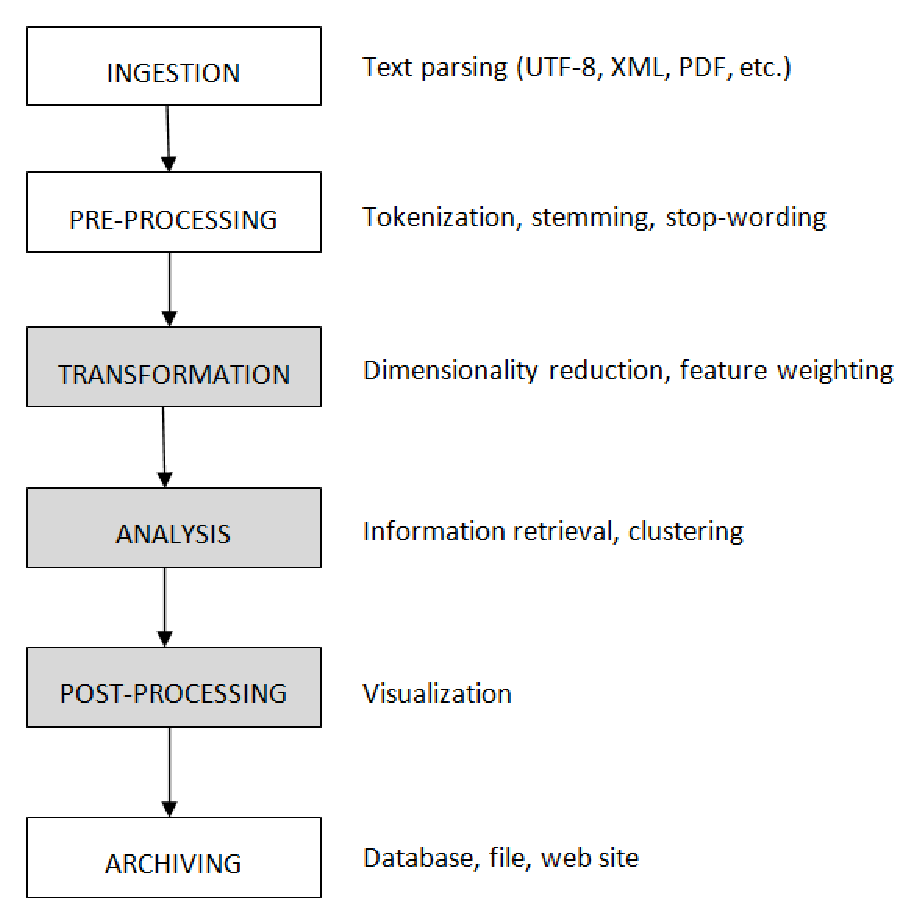
\includegraphics[scale=0.7]{img/text_analysis}
	\caption[Workflow in IR systems]%
           {Workflow in IR systems}
\label{fig:text_analysis}
\end{figure}

Most IR systems share common workflow, and follow common data processing stages. Some of the processes involved in text analysis are: lexical analysis to study word frequency distributions of words, retrieval, tagging/annotation, and visualization among the others. The workflow in \gls{IR} systems usually starts with \textbf{document ingestion}, where texts from the document corpus\footnote{Throughout this work, \emph{document corpus} is used as a synonym to a document collection, in which \gls{IR} tasks are performed.}, which will be analyzed, are parsed or loaded into memory. After that comes the \textbf{preprocessing} phase, responsible for text extraction, tokenization, token-filtering, text folding, etc. In this phase, documents are often represented as vectors, whose components quantify properties like how often words occur in the document. In the \textbf{transformation} phase is where a dictionary, matrix or other form of index is created from the extracted texts. In this phase all extracted terms\footnote{A term in this context denotes a word after preprocessing of the texts. A term is a single unit, e.g. a word, a phrase, a number, or an abbreviation.} are assigned weights by applying a weight function. In Chapter~\ref{sec:lsa:factors_infl_lsa} are given more details about the most common weight functions used in \gls{IR} systems. The \textbf{analysis} phase can include a retrieval process by querying the corpus, clustering, etc. The \textbf{visualization} phase is where concepts, query results, or summarizations extracted from the text collection are presented to users. And in the final \textbf{archiving} phase, results from the text analysis process can be saved.\\


The workflow in fig.~\ref{fig:text_analysis} doesn't show any iterations or cycles between phases for simplicity. Iterations and repetition of certain phases of analysis, however, are common, e.g. between transformation and post-processing phases, or analysis and post-processing. \\

The focus of the current work is on transformation, analysis and post-processing phases of \gls{IR} workflow. 

\section{Goal and scope of work}
\label{sec:goal_scope}
This works contributes with the following:
\begin{enumerate}
\item It  makes an evaluation of Weighted Centroid Covering algorithm, proposed for unsupervised topic labeling of clusters~(\cite{Stein04topicidentification} and \cite{Stein07topicidentification}.
\item It proposes an improvement in \gls{WCC} algorithm, performing topic identification based on external knowledge. A light-weight domain-specific ontology has been developed for this purpose, in order to be used as a reference for external semantic knowledge during cluster labeling. 

\enlargethispage{-\baselineskip}

\item A software application for executing an IR process has been developed. It implements \gls{LSA} for information retrieval~(analysis phase from fig.~\ref{fig:text_analysis}), and presents the main concepts contained in a document set using a tag cloud. \\
\end{enumerate}


\section{Outline}
This chapter motivates the presented work, and summarizes its contributions. It also offers a general overview of the phases of text analysis, common to most \gls{IR} systems. Chapter 2 gives theoretical foundations for preprocessing and transformation phases of text analysis, and reviews a specific technique for information retrieval, called Latent Semantic Analysis. In Chapter 3, \gls{WCC} algorithm is evaluated, and a proposition for its improvement is made, by using a light-weight domain-specific ontology. Chapter 4 refers to the post-processing phase of text analysis, giving the visualization means to present the main concepts retrieved from a document set as a tag cloud. The software contribution, developed as a part of this work, is described in Chapter 5, where test results are also present, and an evaluation of the implementation is made. Finally, in Chapter 6 the thesis concludes with ideas for future work.\\

